\documentclass[10pt]{article}
\usepackage[latin1]{inputenc}

\setlength{\oddsidemargin}{0cm}
\setlength{\evensidemargin}{0cm}
\setlength{\marginparwidth}{0cm}
\setlength{\marginparsep}{0cm}
 
\setlength{\topmargin}{0cm}
\setlength{\textheight}{23cm}
\setlength{\textwidth}{15.6cm}

\usepackage{tikz}

\usepackage{verbatim}
\usetikzlibrary{arrows,shapes}


%\usepackage[english]{babel}
%\usepackage[latin1]{inputenc}
%\usepackage{times}
%\usepackage[T1]{fontenc}

\title{Aritmética}

\author{Daniel Fridlender}

\date{15 de mayo de 2021}


\begin{document}


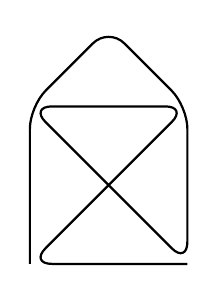
\begin{tikzpicture}
\tikz \draw[thick,rounded corners = 8pt]
    (0,0)-- (0,2)-- (1,3)-- (2,2)-- (2,0)-- (0,2)-- (2,2)-- (0,0)-- (2,0);
\end{tikzpicture}



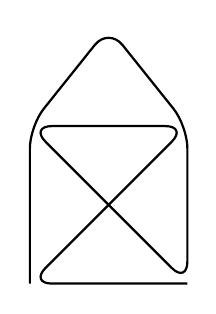
\begin{tikzpicture}
\tikz \draw[thick,rounded corners = 8pt]
    (0,0)-- (0,2)-- (1,3.25)-- (2,2)-- (2,0)-- (0,2)-- (2,2)-- (0,0)-- (2,0);
\end{tikzpicture}


\end{document}